\chapter{Results}
\label{ch:results}

This chapter answers the research questions in order. Every number in it is produced by a
script in the repository and is reproducible from the corpus file
\texttt{data/final/corpus\_naa.csv}; none is transcribed by hand. Where the design cannot
support a claim, the chapter says so at the point the number appears rather than deferring
it to the limitations section.

One convention is fixed before any result: no value of $\hat{\alpha}$ appears anywhere in
this document. Section~\ref{sec:rq3} explains why the coupling is unidentified rather than
merely uncertain.

\section{The corpus as scanned}

The corpus is 400 text items in four categories of 100. All 400 were scanned; the output was
verified row for row against the source corpus on text, category and identifier before any
analysis was run, using \texttt{scripts/verify\_scan\_output.py}.

\begin{table}[htbp]
\centering
\begin{tabular}{@{}lrrr@{}}
\toprule
\textbf{Category} & \textbf{n} & \textbf{Mean} & \textbf{SD} \\
\midrule
Fear activating        & 100 & $-0.0018$ & $0.0204$ \\
High outrage           & 100 & $-0.0185$ & $0.0208$ \\
Neutral informational  & 100 & $-0.0191$ & $0.0162$ \\
Reward hook            & 100 & $-0.0128$ & $0.0228$ \\
\bottomrule
\end{tabular}
\caption{Signed index by category over all 400 scanned items. Every category mean is negative, so deliberative activation leads throughout.}
\label{tab:category-descriptives}
\end{table}

Two features of this table matter before any test is applied. Every category mean is
negative, so the deliberative-control network is predicted to respond more strongly than the
affective-salience network for all four categories; the categories differ in how far below
zero they sit, not in which network leads. And the standard deviations are of the same order
as the differences between the means, which is the reason the separation test in
Section~\ref{sec:rq2} is reported with an effect size rather than a $p$-value alone.

\section{RQ I: the instrument and its classifier performance}
\label{sec:rq1}

\subsection{The ratio form is undefined on real content}

Equation~(4) of the proposal defines the index as a ratio, $A_{\mathrm{aff}} /
(A_{\mathrm{del}} + \delta)$. The encoder emits standardised activation, so an ROI mean sits
near zero and is negative about as often as positive, and the ratio then sign-flips or
diverges. On the completed corpus the ratio is undefined for \textbf{69 of 400 items}, a rate
of $17.25\%$. Those items are counted and reported, never dropped or filled.

The measurement therefore uses the signed difference,
\begin{equation}
\mathrm{NAA}_{\text{signed}} = A_{\mathrm{aff}} - A_{\mathrm{del}},
\end{equation}
which is defined everywhere and is what the field mapping in Chapter~3 requires: the Landau
field needs a signed scalar, not a dimensionless ratio. The classification banding follows
the same constraint. The signed form supports a two-way split on sign, and no magnitude
threshold has been established from any corpus, so the three-band scheme of the proposal
becomes two bands.

\subsection{Classifier performance}

Scored against the \texttt{manipulative} label the items carried before they were ever
scanned, over 300 labelled manipulative and 100 labelled neutral:

\begin{table}[htbp]
\centering
\begin{tabular}{@{}lr@{}}
\toprule
\textbf{Metric} & \textbf{Value} \\
\midrule
AUC (headline)              & $0.6274$ \\
F1 (threshold fitted in sample) & $0.6680$ \\
Precision at that threshold & $0.8426$ \\
Recall at that threshold    & $0.5533$ \\
\bottomrule
\end{tabular}
\caption{Classifier performance against the pre-scan manipulative label. AUC is the headline figure; the threshold behind F1 was fitted in sample and F1 is labelled accordingly.}
\label{tab:classifier}
\end{table}

\textbf{AUC is the headline and F1 is not.} The threshold that produces F1 is chosen on the
same data it is scored on, which inflates it; AUC is threshold-free and does not reward that
choice. A null corpus can return a respectable F1 at an AUC below chance, so quoting F1
alone would present a failure as a success.

The measured AUC of $0.6274$ clears $0.5916$, the smallest AUC this design could detect at
$80\%$ power (Section~\ref{sec:power}), and it lies in the direction the proposal predicted.
It is nonetheless a modest separation, and no per-item verdict is derived from it in this
work: at this AUC, a correct-or-incorrect label on individual items would overstate what the
measurement supports.

\subsection{What a bag of words does on the same label}
\label{sec:baselines}

An AUC has no meaning in isolation. The first question a reader should ask is whether a
lexical model, costing no GPU time at all, does better on the same rows and the same label.
It does, and by a wide margin.

Two baselines were run with \texttt{scripts/baselines.py}: TF-IDF over unigrams and bigrams
with logistic regression, scored on out-of-fold predictions from five-fold stratified
cross-validation, and a sentiment score, the VADER compound valence \cite{hutto2014}, used directly as a score
with nothing fitted. Confidence intervals are $2{,}000$-draw bootstrap percentile intervals on
the same rows.

\begin{table}[htbp]
\centering
\begin{tabular}{@{}llrrl@{}}
\toprule
\textbf{Model} & \textbf{Split} & \textbf{n} & \textbf{AUC} & \textbf{95\% CI} \\
\midrule
NAA signed index     & none, nothing fitted & 400 & $0.6274$ & $[0.5702, 0.6867]$ \\
VADER compound       & none, nothing fitted & 400 & $0.5392$ & $[0.4757, 0.6035]$ \\
VADER $|$compound$|$ & none, nothing fitted & 400 & $0.5300$ & $[0.4693, 0.5923]$ \\
TF-IDF + logistic    & 5-fold stratified    & 400 & $0.9758$ & $[0.9601, 0.9879]$ \\
\midrule
NAA signed index     & ISOT only            & 150 & $0.7290$ & $[0.6431, 0.8132]$ \\
VADER compound       & ISOT only            & 150 & $0.4019$ & $[0.3098, 0.4943]$ \\
TF-IDF + logistic    & ISOT only, 5-fold    & 150 & $0.9724$ & $[0.9483, 0.9901]$ \\
\bottomrule
\end{tabular}
\caption{Baselines against the same manipulative label. The lower block restricts the corpus to the 150 items drawn from the ISOT collection, the only origin corpus contributing both classes.}
\label{tab:baselines}
\end{table}

\textbf{The lexical baseline wins, and the sentiment baseline does not.} TF-IDF reaches
$0.9758$ against the index's $0.6274$, and the two intervals are nowhere near overlapping. The
sentiment score does not clear chance: its interval spans $0.5$ on the full corpus, and on the
restricted set it lies wholly below $0.5$, so there it ranks the label the wrong way round. No claim that the index is a better detector of manipulative content
than counting words is made anywhere in this thesis, and this table is here so that the claim
cannot be read in by implication.

Two qualifications belong with the number rather than after it. The first is that
leave-one-source-out, the obvious correction for the confound of \S\ref{sec:confound}, is not
available: every source dataset in the corpus contributes exactly one class, so a held-out
source leaves a single-class test fold and no per-fold AUC exists. The restricted block is the
available substitute. ISOT-true and ISOT-fake come from one collection, so a model scored on
those 150 items cannot win by recognising which corpus a row came from, and TF-IDF stays at
$0.9724$ there. Its advantage over the index is therefore not only the cross-corpus confound.

The second is that both TF-IDF figures sit above $0.95$, the level at which this project's own
validation module flags a result as more likely a leak than a discovery
(\texttt{app/services/validation.py}). The ISOT true/fake split is known to carry a wire-service
dateline artifact, which the corpus builder strips and verifies, and a near-ceiling lexical
result on a 150-item split is the signature that some residual stylistic marker survives it. A
probe trained on the same features to recover \texttt{source\_dataset} itself, rather than the
label, reaches $66.25\%$ accuracy against a $25\%$ chance rate, which confirms the vocabulary
is substantially source-diagnostic.

What the comparison establishes is therefore narrow, and it is the honest reading: on this
corpus a lexical model separates the label far better than the index does, and a good part of
what it separates is provenance. The index is carried forward here as the field observable
Chapter~3 requires, not as a competitive classifier.

\section{RQ II: distribution across categories}
\label{sec:rq2}

A one-way analysis of variance across the four categories gives
\begin{equation}
F = 15.779, \qquad p = 1.035\times 10^{-9}, \qquad \eta^2 = 0.1068 .
\end{equation}
The effect is roughly four times the $\eta^2 = 0.0268$ the design was powered to detect, and
power at the observed value is $1.0$. The categories separate, and this is not the null that
both partial runs pointed toward.

The separation is not evenly distributed. Welch tests of each category against the neutral
baseline give:

\begin{table}[htbp]
\centering
\begin{tabular}{@{}lrrr@{}}
\toprule
\textbf{Category vs neutral} & \textbf{t} & \textbf{p} & \textbf{Cohen's d} \\
\midrule
Fear activating & $+6.639$ & $3.283\times 10^{-10}$ & $+0.939$ \\
Reward hook     & $+2.254$ & $2.539\times 10^{-2}$  & $+0.319$ \\
High outrage    & $+0.212$ & $8.320\times 10^{-1}$  & $+0.030$ \\
\bottomrule
\end{tabular}
\caption{Welch comparisons of each category against neutral informational. The separation is carried by fear-activating content; high outrage does not separate, and it is the category the proposal expected to separate most.}
\label{tab:welch}
\end{table}

High outrage does not separate from neutral at all. That is the category the proposal
expected to separate most strongly. Fear-activating content carries the result almost
entirely, with reward-hook content contributing a small effect.

\begin{figure}[htbp]
\centering
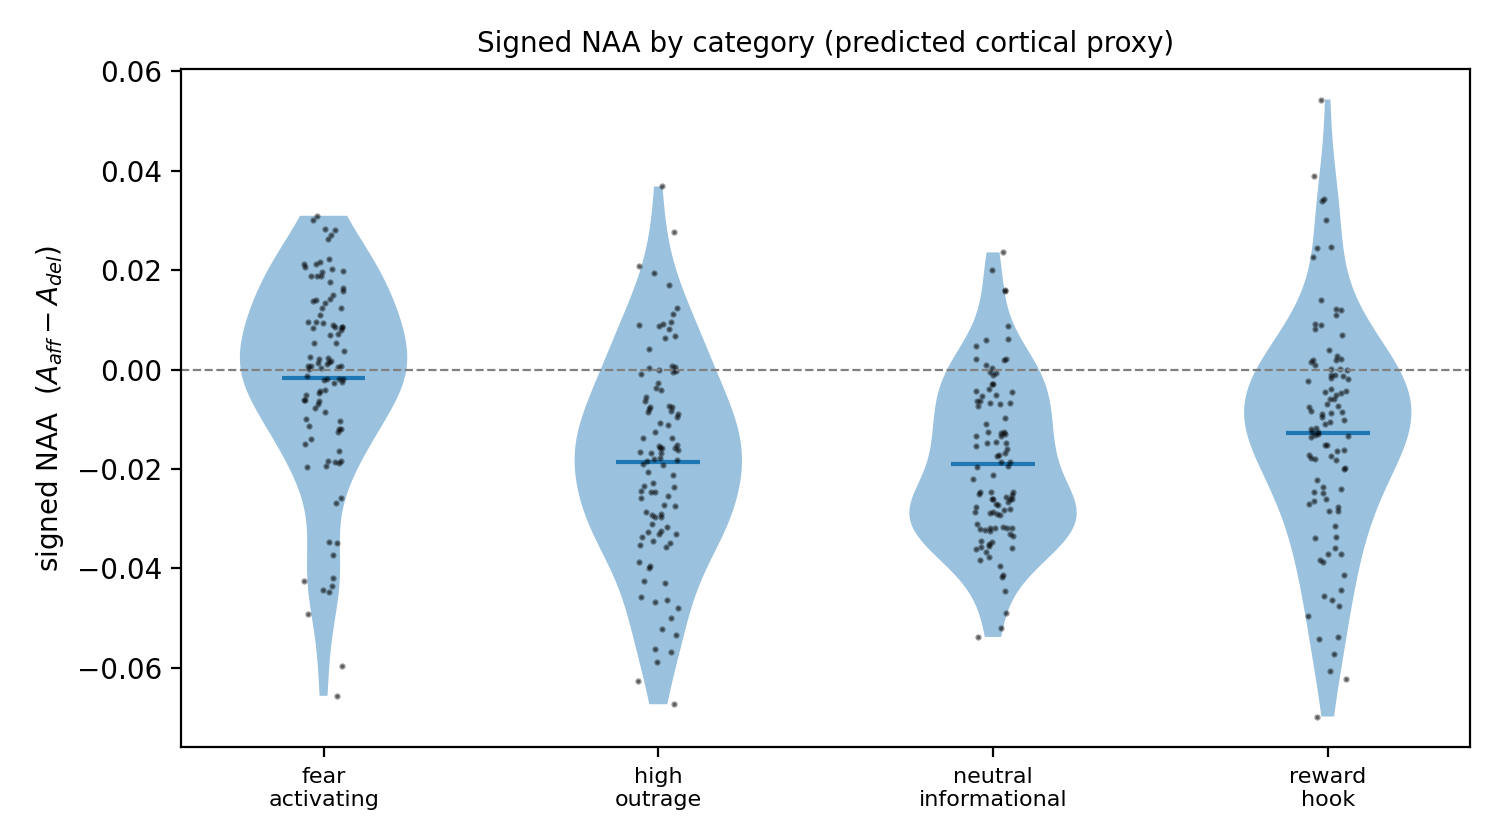
\includegraphics[width=0.9\textwidth]{../../services/inference/data/final/report/fig_violin.png}
\caption{Distribution of the signed index by category over all 400 items.}
\label{fig:violin}
\end{figure}

\begin{figure}[htbp]
\centering
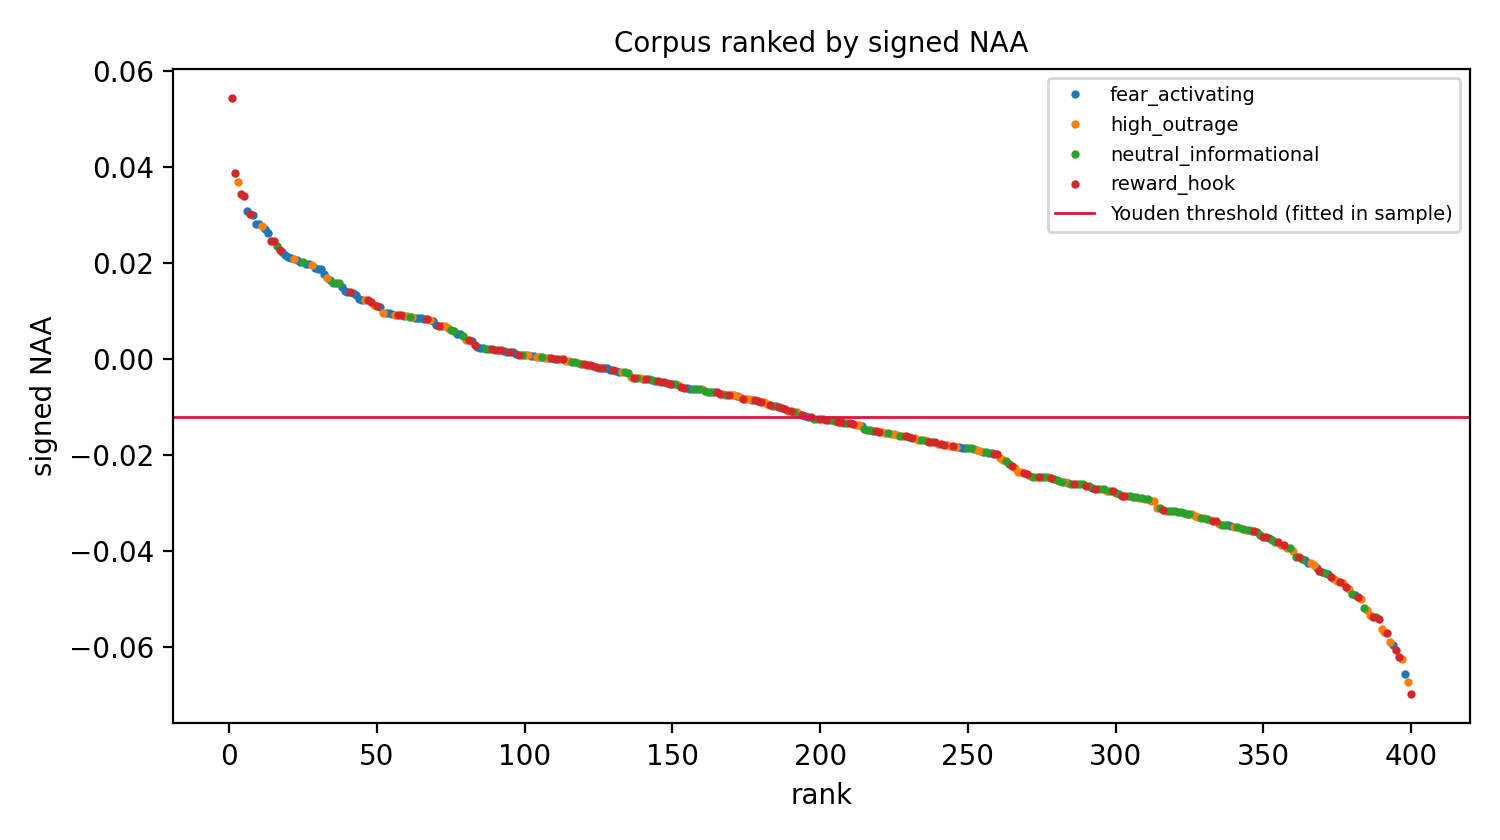
\includegraphics[width=0.9\textwidth]{../../services/inference/data/final/report/fig_ranked.png}
\caption{Every item ranked by the signed index, coloured by category.}
\label{fig:ranked}
\end{figure}

\subsection{The two components, taken separately}
\label{sec:components}

The signed index is a difference, and a difference discards information the corpus already
holds. $A_{\mathrm{aff}}$ and $A_{\mathrm{del}}$ are recorded per item, so each can be compared
against the neutral baseline on its own. This matters for high outrage in particular, where a
large symmetric response and no response are indistinguishable in a difference.

\begin{table}[htbp]
\centering
\begin{tabular}{@{}lrrr@{}}
\toprule
\textbf{Category} & $A_{\mathrm{aff}}$ & $A_{\mathrm{del}}$ & \textbf{signed} \\
\midrule
Fear activating       & $0.03206$ & $0.03385$ & $-0.00179$ \\
High outrage          & $0.02869$ & $0.04719$ & $-0.01850$ \\
Neutral informational & $0.01699$ & $0.03605$ & $-0.01906$ \\
Reward hook           & $0.02310$ & $0.03585$ & $-0.01275$ \\
\bottomrule
\end{tabular}
\caption{Category means of each component and of their difference, over all 400 items.}
\label{tab:components}
\end{table}

\begin{table}[htbp]
\centering
\begin{tabular}{@{}llrrr@{}}
\toprule
\textbf{Category vs neutral} & \textbf{Component} & \textbf{t} & \textbf{p} & \textbf{Cohen's d} \\
\midrule
Fear activating & $A_{\mathrm{aff}}$ & $+4.333$ & $2.365\times 10^{-5}$  & $+0.613$ \\
Fear activating & $A_{\mathrm{del}}$ & $-0.696$ & $4.875\times 10^{-1}$  & $-0.098$ \\
Fear activating & signed             & $+6.639$ & $3.283\times 10^{-10}$ & $+0.939$ \\
\midrule
High outrage    & $A_{\mathrm{aff}}$ & $+3.584$ & $4.263\times 10^{-4}$  & $+0.507$ \\
High outrage    & $A_{\mathrm{del}}$ & $+3.468$ & $6.521\times 10^{-4}$  & $+0.491$ \\
High outrage    & signed             & $+0.212$ & $8.320\times 10^{-1}$  & $+0.030$ \\
\midrule
Reward hook     & $A_{\mathrm{aff}}$ & $+1.842$ & $6.691\times 10^{-2}$  & $+0.261$ \\
Reward hook     & $A_{\mathrm{del}}$ & $-0.063$ & $9.501\times 10^{-1}$  & $-0.009$ \\
Reward hook     & signed             & $+2.254$ & $2.539\times 10^{-2}$  & $+0.319$ \\
\bottomrule
\end{tabular}
\caption{Welch comparisons of each component against neutral informational. High outrage moves both components by nearly the same amount and the difference between them by nothing; fear-activating content moves one component only.}
\label{tab:component-welch}
\end{table}

\textbf{High outrage is not a null in the components.} It raises $A_{\mathrm{aff}}$ by
$d = +0.507$ and $A_{\mathrm{del}}$ by $d = +0.491$, both at $p < 10^{-3}$, and it moves the
difference between them by $d = +0.030$ at $p = 0.832$. The two effects sit within four
hundredths of a standard deviation of each other. The category that fails to separate on the
index is the category that moves both networks together.

Fear-activating content behaves differently in exactly the way that reading predicts. It
raises $A_{\mathrm{aff}}$ by $d = +0.613$ and leaves $A_{\mathrm{del}}$ where it was
($d = -0.098$, $p = 0.488$), so the whole of its $d = +0.939$ on the index is a one-sided
movement. Reward-hook content sits between the two, with a small one-sided lift that does not
reach significance on its component alone.

The pattern holds at the level of the whole design. A one-way analysis of variance on each
component separately gives $F = 7.451$, $p = 7.276\times 10^{-5}$ for $A_{\mathrm{aff}}$ and
$F = 6.399$, $p = 3.052\times 10^{-4}$ for $A_{\mathrm{del}}$, against $F = 15.779$,
$p = 1.035\times 10^{-9}$ for the difference. Both components vary by category; the difference
varies more, because for two of the four categories one component moves while the other holds
still.

\begin{figure}[htbp]
\centering
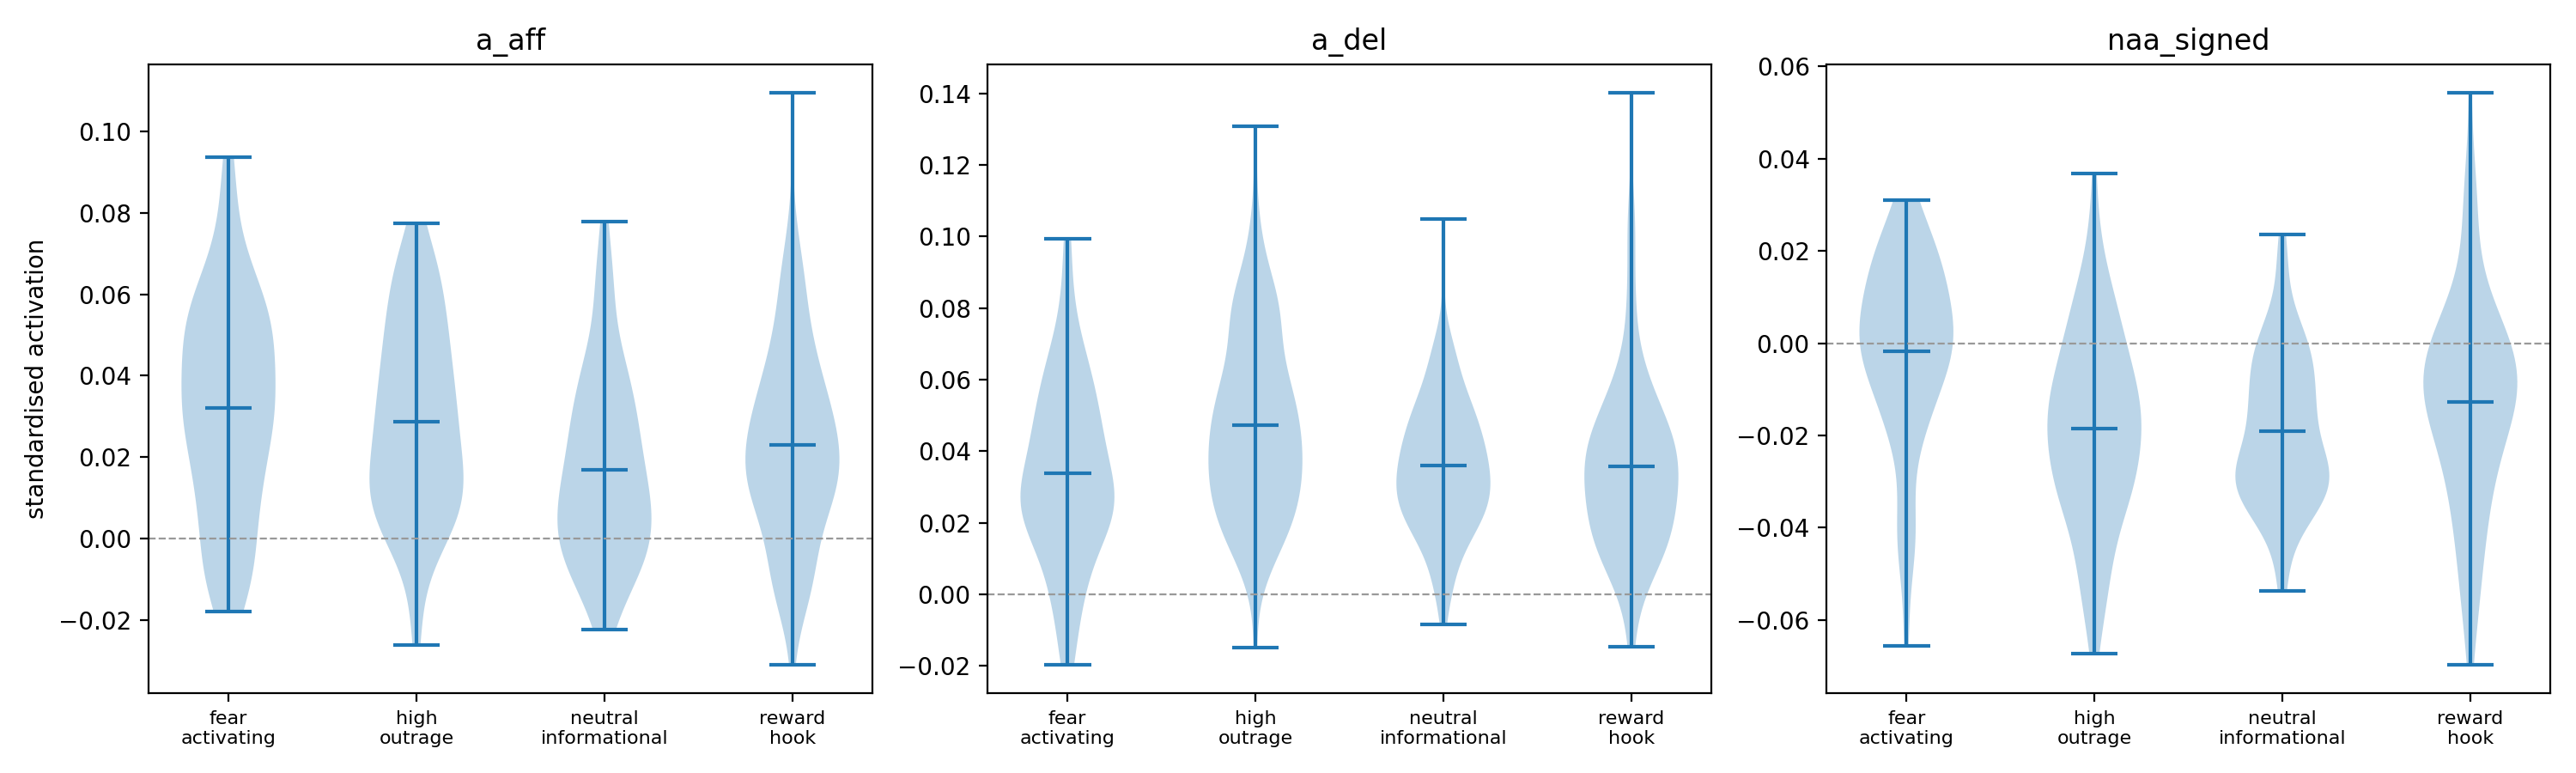
\includegraphics[width=0.95\textwidth]{../../services/inference/data/final/report/fig_components.png}
\caption{$A_{\mathrm{aff}}$, $A_{\mathrm{del}}$ and their signed difference by category over all 400 items. High outrage is elevated on both components and flat on the difference.}
\label{fig:components}
\end{figure}

This does not resolve the confound below, and it says nothing about whether the encoder tracks
cortex. What it does is remove one of the three readings of the outrage null from the list of
things this design cannot distinguish, which \S\ref{sec:outrage} takes up.

\subsection{The confound, stated before the interpretation}
\label{sec:confound}

Each category is drawn from exactly one source dataset: fear-activating from ISOT-fake, high
outrage from SemEval-2019 Task~4, reward-hook from Webis-Clickbait-17, and neutral from
PubMed and ISOT-true in equal parts. Category and provenance are therefore confounded by
construction, and the separation reported above is a separation \emph{between corpora}. It
cannot be attributed to framing rather than to the writing conventions, vocabulary and
editorial process of the source.

Length is not the confounding variable. Word counts are matched across categories at $167.4$,
$163.5$, $163.7$ and $162.2$ with standard deviations near $11$, which the corpus design
achieved deliberately. Provenance is the variable that was not controlled.

One piece of internal evidence argues against a pure source artifact. High outrage is drawn
from its own distinct source and does not separate from neutral on the index. An effect driven
only by provenance would be expected to move every category away from the baseline, not three
of four in an ordered way. The evidence is weaker than that sentence alone suggests:
\S\ref{sec:components} shows high outrage moving on both components and only the difference
staying flat, so a provenance effect is excluded only if it is assumed to act on one ROI union
at a time. This is suggestive, not decisive.

The design that would settle it is a corpus in which framing varies within a single source,
or in which one source appears in more than one category. Neither exists here, so the
attribution remains open and is carried into the discussion as a limitation rather than
resolved by argument.

\begin{figure}[htbp]
\centering
\includegraphics[width=0.95\textwidth]{../../services/inference/data/figures/B3_per_vertex_fear_activating-0000.pdf}
\caption{Predicted response for one fear-activating item at every one of the $20{,}484$
cortical vertices, on the pial surface. Vertices below the map's 70th percentile are left
unpainted so the anatomy remains readable; the threshold is stated in the figure. This is the
encoder's own output and not a smoothed or interpolated field.}
\label{fig:roi-means}
\end{figure}

\section{RQ III: phase structure and the coupling}
\label{sec:rq3}

The mean-field treatment of Chapter~3 gives the free energy $F(m) = a m^2 + b m^4 - hm$ with
$a = (1 - \beta J)/2$ and $b = 1/12$, coefficients derived from the self-consistency
condition rather than asserted. The phase structure is presented across a range of $\alpha$
and is not evaluated at a fitted value.

\subsection{The coupling is unidentified}

The calibration was run three times: on two partial corpora and on the completed 400 items.
On the partial runs the confidence interval comfortably included zero. On the full corpus it
does not, and the bootstrap over $10{,}000$ replicates places no mass below zero.

That is not a measurement of the coupling, for two reasons stated together because either
alone would be misleading. The fit's held-out $R^2$ is \textbf{negative}, so it predicts less
well than the sample mean on data it has not seen. And the estimate scales inversely with
$\beta J$, which no measurement in this study fixes: halving the assumed coupling strength
roughly doubles the fitted value. A single number would therefore report a choice of
$\beta J$ rather than a property of media.

The coupling is accordingly reported as unidentified, and no value is quoted.

\begin{figure}[htbp]
\centering
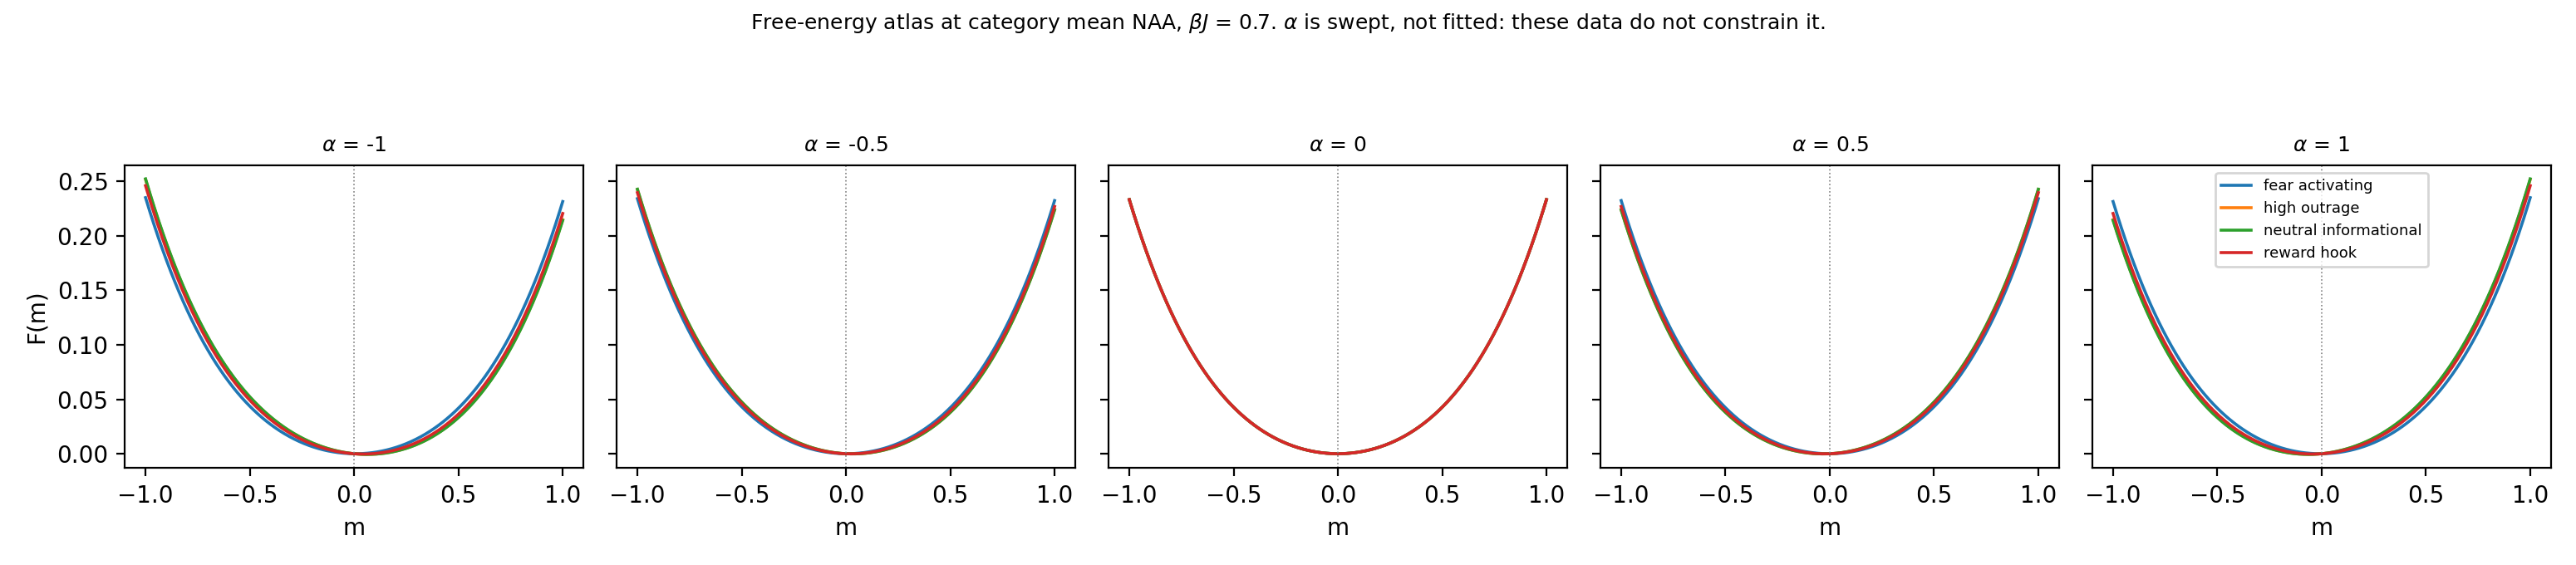
\includegraphics[width=0.9\textwidth]{../../services/inference/data/final/report/fig_free_energy_atlas.png}
\caption{Free energy at each category's measured mean, swept over $\alpha$. The coupling is
swept and never fitted, and no value of $\hat{\alpha}$ is quoted.}
\label{fig:free-energy-atlas}
\end{figure}

\subsection{The bound}

What the corpus does supply is the observable's measured spread, $\Delta X = 0.1241$ over the
range $-0.0698$ to $+0.0543$. Chapter~3's bound,
\begin{equation}
\alpha \;\ge\; \frac{h_c(\beta J)}{\Delta X},
\end{equation}
converts that spread into a statement about what the coupling would have to be:

\begin{table}[htbp]
\centering
\begin{tabular}{@{}lrr@{}}
\toprule
$\beta J$ & $h_c(\beta J)$ & $\alpha$ required \\
\midrule
$1.102$ & $0.02101$ & $0.1693$ \\
$1.496$ & $0.20541$ & $1.6553$ \\
$2.000$ & $0.53284$ & $4.2938$ \\
\bottomrule
\end{tabular}
\caption{The field bound at three values of the reduced coupling. The measured spread $\Delta X = 0.1241$ converts each critical field into the coupling any proposal of this mechanism would require.}
\label{tab:field-bound}
\end{table}

This is a necessary condition and not a sufficient one. Clearing it would not establish that
media of this measured spread moves populations; falling below it excludes the mechanism
within the model's assumptions. The value of the bound is that it requires no fit: it uses
the measured spread and the model's own spinodal, and it applies to any candidate observable
proposed as a field.

\section{Statistical power}
\label{sec:power}

The design's sensitivity was computed before the corpus was analysed and is reported
alongside every result above, so that a reader can see what this study could and could not
have found. At $\alpha = 0.05$ and $80\%$ power, with four categories of 100 and 300 against
100 for the classifier:

\begin{table}[htbp]
\centering
\begin{tabular}{@{}lr@{}}
\toprule
\textbf{Smallest detectable effect} & \textbf{Value} \\
\midrule
Category separation, $\eta^2$ & $0.0268$ \\
Equivalently, Cohen's $f$      & $0.1659$ \\
Classifier AUC                 & $0.5916$ \\
Equivalent separation $d$      & $0.3277$ \\
\bottomrule
\end{tabular}
\caption{Smallest effects this design could detect at $\alpha = 0.05$ and power $0.80$, fixed before the corpus was analysed.}
\label{tab:power}
\end{table}

Both observed effects clear these thresholds, and power at the observed values is $1.0$ for
the separation and $0.961$ for the AUC. Had either fallen below, the correct reading would
have been that the design could not have detected an effect of that size, not that no effect
exists.

\section{RQ IV: out of scope}

Research Question IV asked for per-modality mutual information across text, audio and video.
The amendment reduced the corpus to 400 text items and dropped the audio and video arms, so
the question as posed cannot be answered by this study. The narrowed text-only version was
not reached within the project timeline. It is recorded here as out of scope rather than
attempted and reported thinly.

\section{Summary of the answers}

\begin{enumerate}
\item \textbf{RQ I.} The ratio form of the index is undefined for $17.25\%$ of real content
and is replaced by the signed difference. Against the pre-scan dataset-derived label the index achieves
AUC $0.6274$, above the detectable floor and in the predicted direction, but modest. A TF-IDF
baseline on the same rows reaches $0.9758$, so the index is not the better detector; a
sentiment baseline does not clear chance.

\item \textbf{RQ II.} The four categories separate, $F = 15.779$, $p = 1.035 \times 10^{-9}$,
$\eta^2 = 0.1068$. The effect is concentrated in fear-activating content
($d = +0.939$); high outrage does not separate on the index at all, but raises both component
activations by almost the same amount ($d = +0.507$ and $d = +0.491$), so its flat difference is a
symmetric response rather than an absence of one. Category is confounded with source dataset,
so the separation cannot be attributed to framing.

\item \textbf{RQ III.} The coupling is unidentified and no value is quoted. The measured
spread $\Delta X = 0.1241$ yields a lower bound on any coupling capable of driving a
transition, reaching $\alpha \ge 4.2938$ at $\beta J = 2$.

\item \textbf{RQ IV.} Out of scope under the amendment.
\end{enumerate}

Every category mean remains negative throughout. Whatever the categories differ in, none of
them shows the affective-salience network leading in absolute terms.
